\chapter{Heat pipe temperature model}

In greenhouses the effect of a heat pipe ($E$; \si{W/m}) increases with increasing temperature difference between the warmer pipe ($T$; \si{\degreeCelsius}) and the cooler greenhouse air ($T_a$; \si{\degreeCelsius}). The effect also increases with pipe diameter (inner diameter: $d$; \si{mm}). The relation can be described empirically by
\begin{equation}
  E=ad\left(T-T_a\right)^b
  \label{eq:vg-heat-pipe-E}
\end{equation}
with parameters $a$ and $b$ specific to the pipe material (\iref{fig:vg-heat-pipe-regression}).

\begin{figure} [ht]
\centering
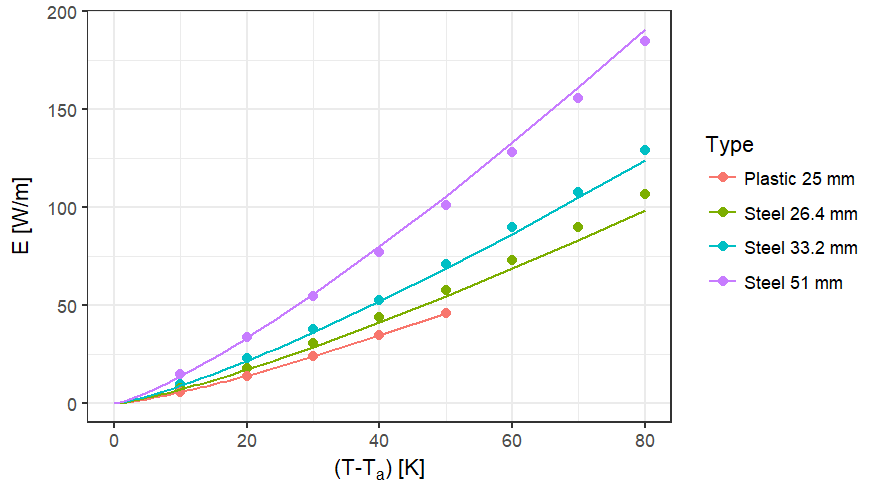
\includegraphics[width=0.67\textwidth]{graphics/vg/heat-pipe-regression.png}
\caption{Regression curves predicting effect ($E$; \si{W} per \si{m} length of pipe) of heat pipes of different materials and diameters \citep[after][Table.~4.3.4]{Braak95}. Curves: $E=ad{\Delta T}^b$. Steel: $a=\SI{0.0154}{W/mm/m}, b=1.253$. Plastic: $a=\SI{0.0123}{W/mm/m}, b=1.281$}
\label{fig:vg-heat-pipe-regression}
\end{figure}

The unit of $a$ is \si{W/mm/m} as we ignore the unit of the exponentiated temperature difference. This is a consequence of the equation resulting from empirical data rather than from physical principles.

The energy lost from the pipe at a rate of $E$ \si{W/m} (remember that \si{W}=\si{J/s}) results from a cooling of the water it contains. As $T$ drops, in the next instance $E$ will drop as well due to the lessened temperature difference, $T-T_a$ (\iref{fig:vg-heat-pipe-regression}). 

Water streams through the pipe and the longer it stays in the pipe, the lower its temperature will drop. For very long heat pipes or very low flow rates, the temperature of the water, as it exits the greenhouse, will approach that of the greenhouse air ($T_a$). Ideally, the temperature of the inflowing water will be regulated to balance the energy lost to the environment and to keep $T_a$ near the current heating setpoint.

We will now reformulate \cref{eq:vg-heat-pipe-E} to express the rate of decline in pipe temperature, \ie\ to let it express \si{K/s/m} instead of \si{W/m}. The specific heat capacity of water is
\[
  C_w = \SI{4.181}{J/cm^3/K} 
\]
The specific heat capacity of water in \SI{1}{m} of pipe is
\[
  C_w V_p \quad[\si{J/K/m}]
\]
where $V_p$ is the volume of water per \SI{1}{m} of pipe,
\[
  V_p = \frac{\pi}{4}d^2 \times \SI{100}{cm} / \SI{1}{m}
\]
For example, taking a pipe with diameter $d=$\SI{35}{mm}, we get
\[
  V_p = \frac{\pi}{4}\left(\SI{3.5}{cm}\right)^2 \times \SI{100}{cm} / \SI{1}{m} = \SI{962}{cm^3/m}
\]
We can then reformulate \cref{eq:vg-heat-pipe-E} as
\begin{equation}
  \frac{dT}{dt} = -\frac{ad}{C_w V_p}\left(T-T_a\right)^b \quad [\si{K/s}] 
  \label{eq:vg-dT-dt}
\end{equation}
To continue the example from above, we have for a \SI{35}{mm} steel pipe:

\begin{align*}
  \frac{dT}{dt} =&\, -\frac{\SI{0.0154}{W/mm/m}\times \SI{35}{mm}}{\SI{4.181}{J/cm^3/K}\times\SI{962}{cm^3/m}}\left(T-T_a\right)^{1.253} \\
                =&\, -0.0001334\left(T-T_a\right)^{1.253} \quad [\si{K/s}]
\end{align*}
The differential \cref{eq:vg-dT-dt} has the solution

\begin{equation}
  T(t) = T_a + \left[ \frac{ad}{C_w V_p}(b-1)t + \left( T(0)-T_a\right)^{1-b}  \right]^\frac{1}{1-b} 
\end{equation}
where $T(0)$ is the initial pipe temperature at time $t=\SI{0}{s}$, and $T(t)$ is the pipe temperature after the passage of $t$ seconds. 

With a water flow rate of $\dot{V}$ (\si{m^3/s}) and a total volume of water in the pipe of $V$ (\si{m^3}), the transit time of water in the pipe (ignoring physical details) is 
\[
  \Delta t = \frac{V}{\dot{V}} \quad [\si{s}]
\]
Or, if water velocity $v$ (\si{m/s}) is known, and total pipe length is $L$ (\si{m}), then
\[
  \Delta t = \frac{L}{v} \quad [\si{s}]
\]


Thus the drop in water temperature from the inflow temperature ($T_{in}$) to the outflow temperature ($T_{out}$) is
\begin{equation}
  \Delta T = T_{in} - T_a - \left[ \frac{ad}{C_w V_p}(b-1)\Delta t + \left( T_{in}-T_a\right)^{1-b}  \right]^\frac{1}{1-b} 
  \label{eq:vg-DT}
\end{equation}
where
\[
  T_{out} = T_{in}-\Delta T
\]

\begin{figure} [ht]
\centering
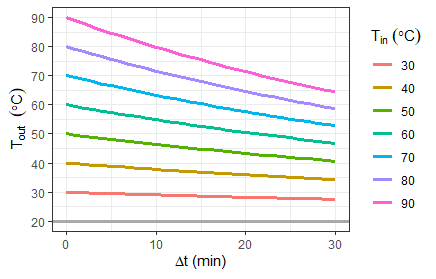
\includegraphics[width=0.67\textwidth]{graphics/vg/heat-pipe-Tout.png}
\caption{Outflow temperature ($T_{out}$) resulting from a range of inflow temperatures ($T_{in}$) and depending on water transit time ($\Delta t$). Other parameter values defined in text.}
\label{fig:vg-heat-pipe-Tout}
\end{figure}

As an example, if a greenhouse is \SI{100}{m} long and \SI{40}{m} wide and has installed one single heat pipe at a density of \SI{1.6}{m} pipe per \SI{1}{m^2} floor area, the total pipe length is
\[
  L = 100\times 40 \times 1.6 = \SI{6400}{m} 
\] 
The total water volume then becomes
\[
  V = \frac{\pi}{4}d^2L = \frac{\pi}{4}\times \left( \SI{0.035}{m}\right)^2 \times \SI{6400}{m} = \SI{6.158}{m^3}
\]
If the flow rate is $\dot{V} = \SI{5}{liter/s}$, we get the transit time of water,
\[
  \Delta t = \frac{\SI{6.158}{m^3}}{\SI{5000}{cm^3/s}} = \SI{1232}{s} = \SI{20.5}{minute}
\]

If we set greenhouse air temperature to $T_a=\SI{20}{\celsius}$ and the inflow temperature to  $T_{in}=\SI{60}{\celsius}$ we can apply \cref{eq:vg-DT} to calculate the temperature drop and the outflow temperature:

\begin{align*}
  \Delta T =&\, \SI{60}{\celsius} - 
              \SI{20}{\celsius} - \\
            \phantom{=}& \left[\SI{0.0001334}{K/s}\,(1.253-1)\SI{1232}{s} + (60-20)^{1-1.253}  
              \right]^\frac{1}{1-1.253}  \\
           =&\, \SI{13.2}{\celsius}
\end{align*}
Thus in this scenario, the outflow temperature has dropped to
\[
  T_{out} = T_{in}-\Delta T = \SI{60}{\celsius}-\SI{13.2}{\celsius} = \SI{46.8}{\celsius}
\]
In \iref{fig:vg-heat-pipe-Tout} other outcomes of the same scenario are shown with varying values of $T_{in}$ and $\Delta t$. 

The total energy emitted by the water is
\begin{align*}
  \Delta E =&\, C_w V \Delta T \\
           =&\, \SI{4.181}{J/cm^3/K} \times \SI{6.158}{m^3} \times \SI{13.2}{K}  \\
           =&\, \SI{338.7}{MJ}
\end{align*}
Thus the average energy flow per floor area becomes
\[
  \frac{\Delta E}{A \Delta t} = \frac{\SI{338.7}{MJ}}{\SI{100}{m}\times\SI{40}{m}\times\SI{1232}{s}} = \SI{68.75}{W/m^2}
\]
This happens to fall within the typical range of the energy demand in a Dutch tomato greenhouse (\iref{fig:vg-heating-demand}).

\begin{figure} [hb]
\centering
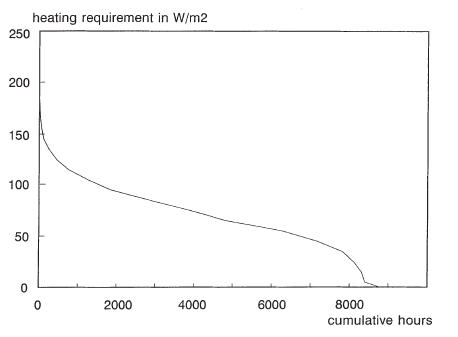
\includegraphics[width=0.5\textwidth]{graphics/vg/heating-demand.png}
\caption{Hourly frequency distribution of heating demand (\si{W/m^2}) over 1 year (\SI{8760}{\hour}) in a Dutch tomato greenhouse  \citep[from][Fig.~4.3.1]{Braak95}.}.
\label{fig:vg-heating-demand}
\end{figure}

\bibliographystyle{plainnat}
\bibliography{nielsholst}
